\chapter{Klasyfikacja tematyczna}
Klasyfikacja tematyczne polega na przypisywaniu jednej lub więcej kategorii/klas danemu dokumentowi. Można to zrobić ręcznie lub algorytmicznie. W tej pracy zebrane zostały dokumenty z portali internetowych, sklasyfikowane ręcznie przez ich autorów. Następnie spróbowano odnaleźć wzorce, którymi kierowano się podczas kategoryzacji oraz podjęto próbę klasyfikacji algorytmicznej. Wyłanianie kategorii na podstawie tekstu ma zastosowanie w wielu dziedzinach, np. w bibliotekoznawstwie, w urzędach lub innych miejscach, gdzie przetwarza się duże ilości danych, których ręczna klasyfikacja jest niemożliwa.\cite{text-classification-stanford} Teksty mogą być klasyfikowane według różnych atrybutów, np.: płci autora, roku wydania, rodzaju dokumentu. W omawianej pracy podjęto próbę wyłonienia odpowiedniej kategorii podanych tekstów. 
\section{Przegląd literatury}
W pracy wykorzystano wiedzę z artykułów oraz książek, które niekoniecznie odnoszą się do przetwarzania tekstu w języku polskim. W większości zaproponowane sposoby klasyfikacji były tożsame, dopóki nie odnosiły się do zagadnień opartych o zasady, którymi kieruje się dany język. Gramatyki dla języka polskiego oraz angielskiego różnią się w znaczący sposób, konieczne zatem było zaproponowanie odpowiednich klas gramatycznych. \cite{polishGrammarTagset} 

\section{Przyjęta terminologia}
Wiele nowych technologii i odkryć dotyczy najczęściej języka angielskiego i to przede wszystkim ten język poddawany jest różnego rodzaju testom, podobnie jest także w odniesieniu do przetwarzania i automatycznej kategoryzacji tekstów. Oczywistą różnicą miedzy językiem polskim, a językiem angielskim jest rozbudowana fleksja w przypadku języka polskiego, co wymagało przekształcenia niektórych terminów. W niniejszej pracy przyjęte terminy zostały zaczerpnięte z literatury skupiającej się głównie na indeksowaniu treści \cite{indeksowanietresci}, te z kolei są przystosowane do języka polskiego bazując na rozwiązaniach stosowanych w języku angielskim oraz wiedzy zawartej w książce \textit{Statystyka dla językoznawców} \cite{stats}. Podstawowe terminy wykorzystane w pracy:

\begin{itemize}
\item \textbf{token} - (segment) najmniejsza niepodzielna jednostka tekstu,
\item \textbf{słowo} - ciąg znaków pomiędzy deliminatorami tekstu,
\item \textbf{słowoforma} - (forma wyrazowa) słowo o przypisanych cechach semantycznych i gramatycznych,
\item \textbf{leksem} - zbiór słowoform, zawierający wszystkie poprawne formy gramatyczne,
\item \textbf{hasło} - (lemat) - jedna zwyczajowo przyjęta forma gramatyczna,
\item \textbf{wyraz} - graficzna postać leksemu, hasła lub słowoformy,
\item \textbf{słowa nierelewantne} (ang. stop words) - wyrazy mało znaczące.
\end{itemize}


\subsection{Analiza morfologiczna}
Morfologia jest nauką o budowie słów. Dziedzina  ta zajmuje się dwiema odrębnymi dziedzinami takimi jak fleksja, która opisuje różne formy danego fleksemu oraz słowotwórstwo, które definiuje zasady tworzenia wyrazów pochodnych. \cite{mykowiecka}
Istotnym aspektem pracy była analiza morfologiczna, która dostarcza potrzebną wiedzę o zadanym tekście. Analiza morfologiczna polega na wyznaczeniu wszystkich form podstawowych dla danego słowa (lematów) oraz wyznaczeniu wszystkich możliwych interpretacji wyznaczonego lematu. Operacją odwrotną do analizy morfologicznej jest synteza morfologiczna, czyli stworzenie wykładnika formy fleksyjnej na podstawie lematu oraz cech fleksyjnych. Kontekst w przypadku analizy morfologicznej nie jest brany pod uwagę. \cite{morfeusz-reference}

\subsection{Segmentacja}
Segmentacja skupia się na podziale tekstu na poszczególne segmenty. Wbrew pozornej niezależności segmentacja jest silnie związana z cechami dla danego języka. Oznacza to, że problem segmentacji nie jest łatwo rozwiązywalny przy pomocy reguły dzielenia tekstu na podstawie odstępów między segmentami. \cite{mykowiecka} Wyróżnić można kilka klas segmentów:
\begin{itemize}
\item ciąg cyfr,
\item ciąg cyfr z wewnętrznym przecinkiem/kropką,
\item ciąg małych liter,
\item ciąg małych liter poprzedzonych wielką literą,
\item ciąg składający się tylko z wielkich liter,
\item znak interpunkcyjny.
\end{itemize}

Do rozpoznawania granic tokenów można zastosować automaty skończone, przykład został pokazany na rysunku \ref{fig:state-machine}. Jest to trudna w realizacji metoda, gdyż wymaga zbioru słowników, zawierających wszystkie formy każdego leksemu. 

\begin{figure}[ht!]
	\centering
	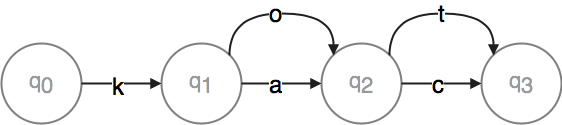
\includegraphics[width=0.6\linewidth]{img/state-machine}
	\caption{Przykład automatu dla fragmentu słownika języka polskiego z formami mianownikowymi wyrazów: kot, kat, koc, kac}
	\label{fig:state-machine}
\end{figure}
% * <jakub.pomykala@gmail.com> 2018-06-10T20:08:48.229Z:
% 
% Ja bym tu dodała krótki opis jak to działa, tzn. opis tego rysunku - w q1 wybiera się lierkę o lub a, później w q2 literkę t lub c i w ten sposób powstaje słowo.
% 
% ^.
 Drugim powszechnie znanym sposobem na segmentację tekstu jest zastosowanie algorytmu regułowego. Opiera się on na zastosowaniu kilku zasad, na podstawie których wyznaczane są zakończenia i rozpoczęcia tekstu oraz potencjalne zakończenia i potencjalne rozpoczęcia tekstu. Potencjalnym zakończeniem tekstu może być skrót, na przykład \textit{inż.}. Mimo, iż zdania zawsze kończone są kropkami, to użycie skrótu \textit{inż.} w zdaniu nie powinno dzielić tego zdania na dwa osobne byty. \cite{rudolf-swidzinski}

\subsection{Lematyzacja}
Celem lematyzacji jest sprowadzanie formy fleksyjnej wyrazu do postaci słownikowej. Zastosowanie form podstawowych w klasyfikacji tekstu ma bardzo dużą zaletę z uwagi na możliwość ograniczenia zbioru, na którym wykonywana jest praca. Dodatkowo umożliwia to traktowanie wszystkich wyrazów, które stanowią odmianę danego zwrotu, jak to samo słowo. W przypadku języka angielskiego, który ma bardzo ubogą fleksję, wyznaczanie form podstawowych może się odbywać, np. na drodze usuwania końcówek wyrazów \textit{-ing} lub \textit{-s}. Język polski ma bardzo bogatą fleksję, dlatego takie podejście zupełnie by się nie sprawdziło. Konieczne zatem było przeprowadzenie kompletnej analizy morfologicznej z wykorzystaniem gotowych narzędzi i bibliotek.

\section{Istniejące rozwiązania}
Podczas wyszukiwania istniejących rozwiązań skupiono się głównie na narzędziach spełniających rolę analizatorów morfologicznych, ponieważ przede wszystkim one będą dostarczać potrzebną wiedzę o tekście. 


\subsection{Morfeusz SGJP}
Morfeusz jest analizatorem morfologicznym dla języka polskiego, który jest najczęściej spotykany w różnego rodzaju pracach. \cite{morfeusz-practical-tool} Dla zadanego ciągu słów potrafi podzielić zdanie na słowa, a następnie zinterpretować każde słowo podając jego klasę gramatyczną i formę podstawową. Każde słowo może mieć więcej niż jedną interpretację, co wynika ze złożoności języka. Tagi zastosowane w programie Morfeusz są pozycyjne. Pierwsza pozycja definiuje część mowy, kolejne oznaczają wartości kategorii gramatycznych każdej klasy. \cite{morfeusz-reference} Program \textit{Morfeusz SGJP} w wersji demo jest dostępny pod adresem \url{http://sgjp.pl/morfeusz/demo} Analizator ten wykorzystuje metodę automatów skończonych do segmentacji tekstu.

\subsection{TaKIPI}
TaKIPI (Tager Korpusu IPI PAN) to narzędzie, które ustala opis morfo-syntaktyczny dla wyrazów w tekście. Program wykorzystuje algorytm regułowy, składający się z niewielkiego zestawu ręcznie stworzonych reguł oraz kilku tysięcy pozyskiwanych automatycznie. Według źródła, skuteczność TaKIPI wynosi około 93.4 procent. \cite{takipi-polish-tagger} TaKIPI wykorzystuje program \textit{Morfeusz} omówiony wcześniej oraz narzędzie \textit{Odgadywacz} do odkrywania opisów morfo-syntaktycznych nieznanych wyrazów i automatycznego budowania wcześniej wspomnianych reguł. \cite{odgadywacz} Oprogramowanie jest rozpowszechniane w postaci programu komputerowego, niestety brak kompatybilności z system \textit{MacOS} sprawił, że nie był on brany po uwagę podczas rozważań na wyborem analizatora. \cite{takipi-polish-tagger}

\subsection{Platforma CLARIN}
CLARIN \cite{clarinMrofeusz2} jest projektem europejskim, który zapewnia zbiór narzędzi do przetwarzania języka w postaci wygodnego interfejsu webowego REST API. Dodatkowym atutem jest mnogość dostępnych konfiguracji oraz przyjmowane formaty danych (np.: pliki *.zip, pliki *.txt lub tekst w zapytaniu POST do serwera i inne). Komunikacja przez API odbywa się w sposób asynchroniczny; oznacza to, że dane najpierw muszą zostać wysłane i zapisane na serwerze, a odwołujemy się do nich przy pomocy ID, które dostajemy w odpowiedzi. Następnie, można użyć dostępnych narzędzi poprzez wysyłanie odpowiednich zapytań HTTP do serwera.

\subsection{Tagger WCRFT2}
Tagger WCRFT2 (Wrocław CRF Tagger) jest jednym z narzędzi dostępnych w Clarin; jest to tagger morfo-syntaktyczny dla języka polskiego. Składa się on z kilku mniejszych programów i technologii takich jak: Corpus2, MACA, Morfeusz SGJP \cite{wcrft} oraz WCCL. Użycie tego narzędzia odgrywa istotną rolę w niniejszej pracy, ponieważ pozwoliło ono na uzyskanie lematów z tekstów oraz wyznaczenie klas gramatycznych dla każdego słowa w prosty sposób. Dostęp do narzędzia można uzyskać przez skompilowanie go na swoim komputerze lub przez API, udostępnione w Clarin. Stworzenie tego narzędzia było zainspirowane przez podobny program o nazwie Wrocław Memory-Based Tagger. WCRFT znajduje się na licencji GNU LGPL v3.0.

